%TODO: example Hinfty
%TODO: old parameter K stuff?

\section{Robust Control}

\subsection{Norms for signals and systems}
The $\mathcal{L}_2$ (euclidian norm) of continuous signal $u$ or a vector-valued signal $\mathbf{u}$ is
\begin{align*}
    ||u||_2 &= \sqrt{\int_{-\infty}^{\infty} u^2(t) dt} &
    ||\mathbf{u}||_2 = \sqrt{\int_{-\infty}^{\infty} \mathbf{u}^T \mathbf{u} dt}
\end{align*}

The $\mathcal{H}_2$ norm of a \emph{stable} system $G(s)$ is defined as the $\mathcal{L}_2$
norm of its impulse response $g(t)$.

The $\mathcal{H}_{\infty}$ norm is defined as the maximum RMS amplification over all arbitrary input signals $u\neq 0$.
This equals the peak magnitude in the Bode diagram of the transfer function $G(j\omega)$.
\[
    ||G||_{\infty} = \sup_{u \in \mathcal{L}_2} \frac{||y||_2}{||u||_2} = \sup_{\omega} |G(j\omega)|
\]

\subsection{The Nyquist Criterion and the Small Gain Theorem}

\begin{minipage}{10cm}
    \paragraph{Nyquist Criterion}The closed loop system with loop gain $L(s)$ and a negative feedback polarity
    is stable if the Nyquist plot of $L(j\omega)$ encircles the critical point $s_{crit}=-1$ exactly
    $N_P$ times anticlockwise, where $N_P$ is the number of unstable poles of $L(s)$.
    
    If $L(s)$ is a stable open loop transfer function, $N_P = 0$.

    \paragraph{Gain Margin, Phase Margin and Critical Distance}
    In robust control, the critical distance $d_{crit}$ is used instead
    of phase and gain margin. 
    \[
        d_{crit} = \min_{\omega} |L(j\omega) - s_{crit}| = \min_{\omega}|1+L(j\omega)|
    \]
    This is the reciprocal of the sensitivity function
    \[
        d_{crit} = \frac{1}{||S||_{\infty}}, \quad \text{where } S(j\omega) = \frac{1}{1 + L(j\omega)}
    \]
\end{minipage}
\hspace{0.5cm}
\begin{minipage}{8cm}
    \centering
    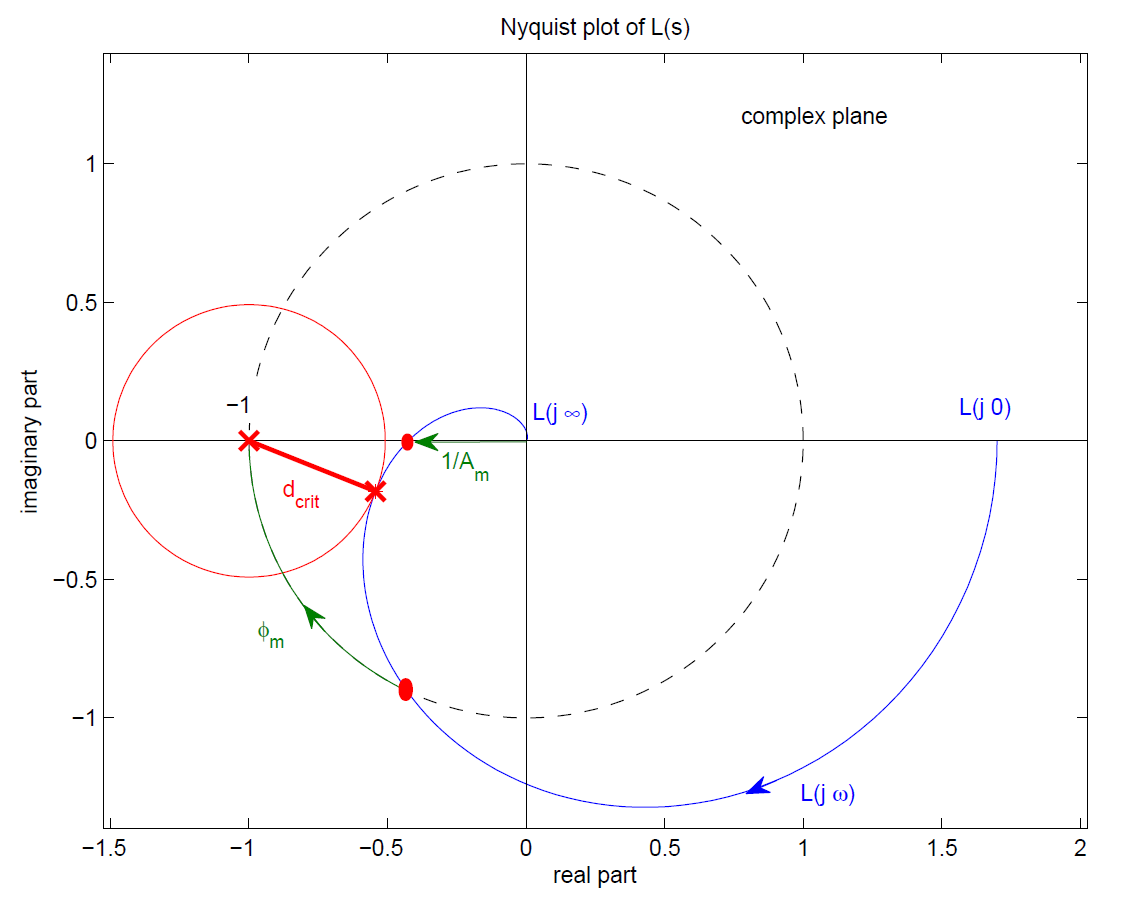
\includegraphics[width=\linewidth]{bilder/robust_nyquist.png}
\end{minipage}

\paragraph{Small Gain Theorem}
If $L(s)$ is stable and $||L||_{\infty} < 1$, then the loop gain $|L(j\omega)|$ is smaller
than $1$ for all frequencies $\omega$.
Hence, $L(j\omega)$ does not encircle the critical point $-1$.
The resulting phase margin is \emph{infinite}: $\phi_m = \infty$.

The small gain condition $||L||_{\infty} < 1$ is \emph{sufficient} but not \emph{necessary}
for closed loop stability.

\begin{minipage}{10cm}
    \paragraph{Application of the Small Gain Theorem}
    For a plant $P(s)$ with a nominal transfer function $P_0(s)$, an additive 
    perturbation $\Delta_a(s)$, and a stabilizing controller $C(s)$, the 
    question arises, how large $\Delta_a(s)$ can become
    before becoming unstable.
    
    The feedback seen by $\Delta_a$ is $\frac{-C}{1+P_0 C}$.
    A sufficient condition for the stability using the small gain theorem is therefore
    \begin{align*}
        \left\lVert \Delta_a \cdot \frac{-C}{1+P_0 C}\right\rVert_{\infty} < 1 && \Leftrightarrow &&
        ||\Delta_a||_{\infty} < \frac{1}{\left\lVert \frac{C}{1+P_0C} \right\rVert_{\infty}}
    \end{align*}
\end{minipage}
\hspace{0.5cm}
\begin{minipage}{8cm}
    \centering
    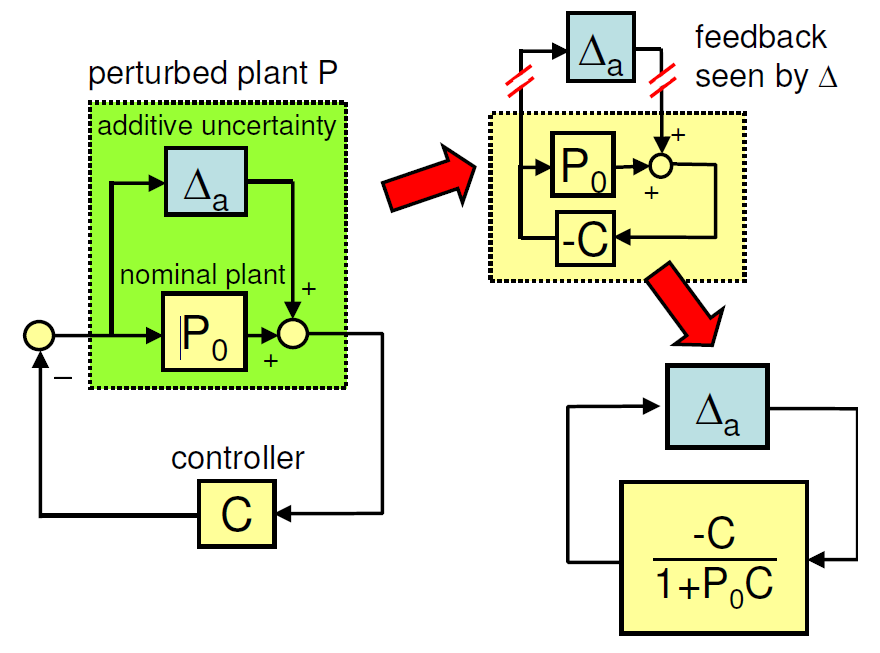
\includegraphics[width=7cm]{bilder/rob_smallgain.png}
\end{minipage}

The Bode integral theorem states that
\[
    \int_{0}^{\infty} \ln |S(j\omega)| d\omega = \pi \sum_{\text{unstable poles $p$ of $L(s)$}} \Re(p)
\]

\subsection{Unstructured Uncertainty}

\begin{minipage}[b]{0.5\linewidth}
    \paragraph{Additive Uncertainty}~\\
    \begin{center}
        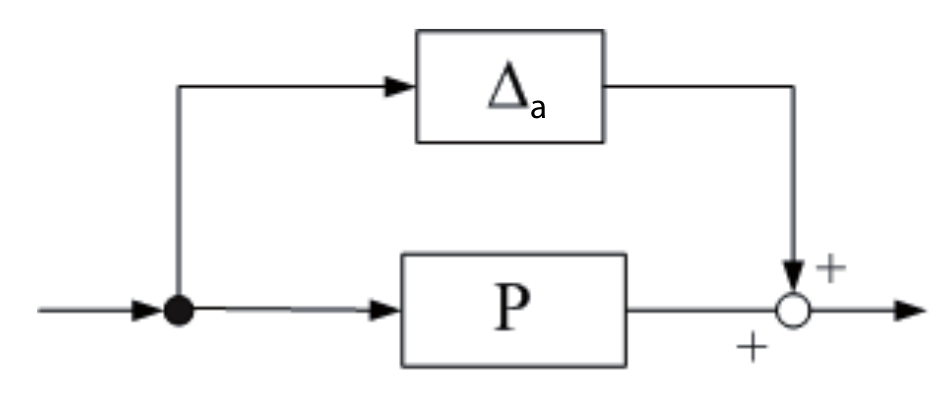
\includegraphics[width=4cm]{bilder/rob_add.png}
    \end{center}
    Transfer function:
    \[
        P(s) = P_0(s) + \Delta_a(s)
    \]
    and
    \[
        \Delta_a(s) = W_{2a}(s) \cdot \tilde{\Delta}_a(s)
    \]
    where $\tilde{\Delta}_a$ is \emph{any} stable, normalized perturbation with
    \[
        ||\tilde{\Delta}_a||_{\infty} \leq 1
    \]
    and the radius is scaled with $W_{2a}(s)$.
    
    From the small gain theorem, the perturbed system is stable if
    \[
        ||\Delta_a||_{\infty} < \frac{1}{\left\lVert\frac{C}{1+P_0C}\right\rVert_{\infty}}
    \]
\end{minipage}
\begin{minipage}[b]{0.5\linewidth}
    \paragraph{Multiplicative Uncertainty}~\\
    \begin{center}
        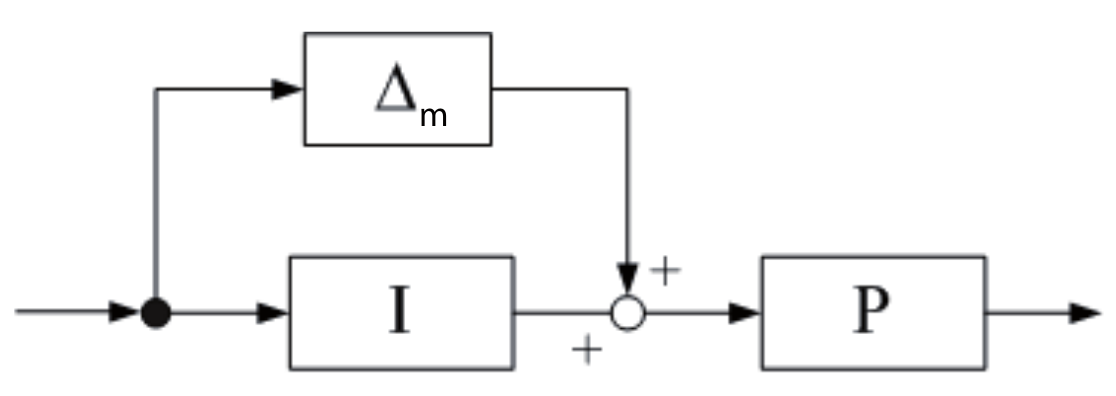
\includegraphics[width=4cm]{bilder/rob_mult.png}
    \end{center}
    Transfer function:
    \[
        P(s) = P_0(s) \cdot (1 + \Delta_m(s))
    \]
    and
    \[
        \Delta_m(s) = W_{2m}(s) \cdot \tilde{\Delta}_m(s)
    \]
    where $\tilde{\Delta}_m$ is \emph{any} stable, normalized perturbation with
    \[
        ||\tilde{\Delta}_m||_{\infty} \leq 1
    \]
    and the radius is scaled with $W_{2m}(s)$.
    
    From the small gain theorem, the perturbed system is stable if
    \[
        ||\Delta_m||_{\infty} < \frac{1}{\left\lVert\frac{P_0C}{1+P_0C}\right\rVert}
    \]
\end{minipage}
\vspace{0.5em}

In the SISO case, additive uncertainty can be recast into multiplicative
uncertainty by
\[
    P_0(s) \Delta_m(s) = \Delta_a(s)
\]

\paragraph{Dead time}An uncertain dead-time can be described as multiplicative uncertainty
\begin{align*}
    P(s) = P_0(s) \cdot e^{-sT} && \Leftrightarrow && \Delta_m(s) = e^{-sT} - 1
\end{align*}

\subsection{Linear Fractional Transformation (LFT)}
\begin{minipage}{12cm}
    The plant can be partitioned according to the dimensions of $\Delta$
    \[
        P = \begin{bmatrix}
            P_{11} & P_{12} \\
            P_{21} & P_{22}
        \end{bmatrix}
    \]
\end{minipage}
\hspace{0.5cm}
\begin{minipage}{6cm}
    \centering
    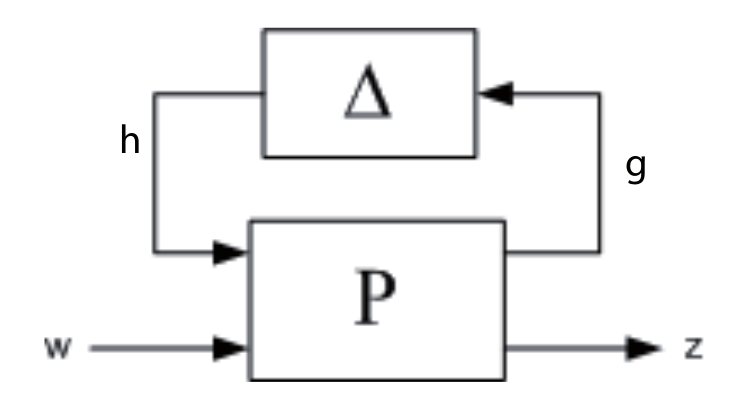
\includegraphics[width=4cm]{bilder/rob_lft.png}
\end{minipage}

which corresponds to
\[
    z = \left( P_{22} + P_{21} \Delta(I-P_{11}\Delta)^{-1} P_{12} \right) w
\]
We define the \emph{linear fractional transformation} (LFT) of $P$ and $\Delta$ as
\[
    \mathcal{F}(P,\Delta) = P_{22} + P_{21} \Delta (I-P_{11}\Delta)^{-1} P_{12}
\]

Additive and multiplicative uncertainties are special cases of the LFT:
\begin{align*}
    \text{Additive:} \quad
    P = \begin{bmatrix}
        0 & I \\ I & P_0
    \end{bmatrix}
    &&
    \text{Multiplicative:} \quad
    P = \begin{bmatrix}
        0 & P_0 \\ I & P_0
    \end{bmatrix}
\end{align*}

\subsection{Structured Uncertainty}
Concrete physical parameters and tolerances can be modeled using structured uncertainties.
A structured uncertainty leads to a \emph{static diagonal} block $\Delta$. The diagonal
elements are \emph{real-valued}.
(In contrast to mostly complex-valued, norm-bounded transfer functions $\Delta(s)$ as in unstructured uncertainties.)

\subsection{The Standard $\boldsymbol{\mathcal{H}}_{\boldsymbol{\infty}}$ Problem}
The $\mathcal{H}_{\infty}$ design is to create robust controllers. 
A system which is stable with all possible uncertainties of a plant is called
\emph{robustly stable}.

From the small gain theorem, it follows that a system is robustly stable, if
\begin{align*}
    \text{Additive:}\quad&
    ||W_2 C(I+PC)^{-1}||_{\infty} \leq 1 \\
    \text{Multiplicative:}\quad&
    ||W_2 PC(I+PC)^{-1}||_{\infty} \leq 1
\end{align*}
Further, the sensitivity function $S=(I+PC)^{-1}$ must meet the condition
\begin{align*}
    || \gamma W_1 (I+PC)^{-1} ||_{\infty} \leq 1 
    && \Rightarrow &&
    S(j\omega) \leq \frac{1}{|W_1(j\omega)|}
\end{align*}
where $\gamma$ is an optimization parameter. 
The larger $\lambda$, the better the disturbance attenuation.
A controller is now created by solving the optimization problem:
\begin{align*}
    \text{Additive:}\quad&
    \max_{\lambda} \left\lVert \begin{bmatrix}
        \lambda W_1(s) (I+PC)^{-1} \\
        W_{2a}(s) C (I+PC)^{-1}
    \end{bmatrix} \right\rVert_{\infty} = 1
    \\
    \text{Multiplicative:}\quad&
    \max_{\lambda} \left\lVert \begin{bmatrix}
        \lambda W_1(s) (I+PC)^{-1} \\
        W_{2m}(s) PC (I+PC)^{-1}
    \end{bmatrix} \right\rVert_{\infty} = 1
\end{align*}
This is equivalent to finding a controller $C$, for which
\[
    ||\mathcal{F}(P,C)||_{\infty} = ||P_{11} + P_{12}C(I-P_{22}C)^{-1} P_{21}||_{\infty} = 1
\]

\paragraph{State Space Solution}~\\
\begin{minipage}{10cm}
    The state space representation is
    \begin{align*}
        \dot{x} &= Ax + B_1 w + B_2 u \\
        z &= C_1 x + D_{11} w + D_{12} u \\
        y &= C_2 x + D_{21}w + D_{22} u
    \end{align*}
    with the general system matrix
    \[
        G_s = \begin{bmatrix}
            A & \vdots & B_1 & B_2 \\
            \dots & & \dots & \dots \\
            C_1 & \vdots & D_{11} & D_{12} \\
            C_2 & \vdots & D_{21} & D_{22}
        \end{bmatrix}
    \]
\end{minipage}
\hspace{0.5cm}
\begin{minipage}{8cm}
    \centering
    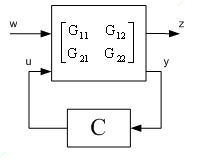
\includegraphics[width=4cm]{bilder/hinf_statespace.png}
\end{minipage}

An optimal closed solution for the general system is not known. 
A closed solution for the following special case does exist:
\[
    G_s = \begin{bmatrix}
        A & \vdots & B_1 & B_2 \\
        \dots & & \dots & \dots \\
        C_1 & \vdots & 0 & \begin{bmatrix}0\\I\end{bmatrix} \\
        C_2 & \vdots & \begin{bmatrix}0&I\end{bmatrix} & 0
    \end{bmatrix}
\]
Among other conditions, the $\mathcal{H}_{\infty}$ problem must have
a solution at $\omega = \infty$. The weighting functions $W$ must ensure this.
